\begin{exercice}
Antoine possédait 832,25 CHF sur son livret d'épargne. Pour son anniversaire, ses parents y ont déposé 75 CHF. Combien a-t-il maintenant sur son livret ?
\end{exercice}


\begin{exercice}
Un panier plein de fruits pèse 1,836 kg. Vide, il pesait 0,425 kg. Quelle est la masse des fruits contenus dans ce panier ?
\end{exercice}


\begin{exercice}
Pierre a relevé le compteur de sa voiture au départ et au retour de vacances. Au départ, le compteur indiquait 58\,257,6 km. Au retour, il indiquait 59\,329,1 km. Quelle distance a‑t‑il parcourue pendant ses vacances ?
\end{exercice}


\begin{exercice}
Simon veut acheter un livre. Il a 25,35 CHF dans son porte‑monnaie et il lui manque 5,25 CHF pour acheter ce livre. Quel est le prix du livre ?
\end{exercice}


\begin{exercice}
Une voiture consomme 8,5 l d'essence pour faire 100 km. Combien d'essence consomme‑t‑elle pour faire 500 km ?
\end{exercice}
  
  
\begin{exercice}
Un employé gagne 17,25 CHF de l'heure. Il travaille 35 heures par semaine. Combien gagne‑t‑il chaque semaine ?
\end{exercice}


\begin{exercice}
Au marché, Anne a déposé dans son panier 1,2 kg de carottes, 600 g de raisin et 1,3 kg de pommes. Combien pèse le contenu de son panier ?
\end{exercice}


\begin{exercice}
Pour aller au collège, Caroline fait 1,4 km avec son vélo qu'elle laisse chez sa grand‑mère. Puis elle parcourt 150 m à pied jusqu'au collège. Quelle distance totale parcourt‑elle pour se rendre au collège ?
\end{exercice}


\begin{exercice}
Djamel a acheté 1,6 kg de poires à 2,30 CHF le kg. Combien a‑t‑il payé ?
\end{exercice}


\begin{exercice}
Gérard a payé 41,40 CHF pour 12 pieds de tomate. Quel est le prix d'un pied de tomate ?
\end{exercice}



\begin{exercice}
Un lot de six stylos identiques coûte 8,10 CHF. Quel est le prix d'un stylo ?
\end{exercice}


\begin{exercice}
Mercredi après‑midi, Anh Hao a fait cinq tours d'un circuit de VTT. Il a parcouru en tout 23,5 km. Quelle est la longueur de ce circuit ?
\end{exercice}


\begin{exercice}
Mme Betty possède 6,6 litres de jus de pomme. Combien de bouteilles de 0,7 litres pourra-t-elle remplir ?
\end{exercice}

\begin{exercice}
Agan possède 37,40 CHF en pièces de 20 centimes. Combien de pièces de 20 centimes possède t'il ?
\end{exercice}


\begin{exercice}[Énigme]
Trouve le nombre décimal à six chiffres tel que :
\begin{itemize}
 \item son chiffre des unités est 2 ;
 \item l'un de ses chiffres est 6 et sa valeur dans l'écriture décimale est cent fois plus petite que celle du chiffre 2 ;
 \item son chiffre des dizaines est le double de celui des unités et son chiffre des dixièmes est le quart de celui des dizaines ;
 \item ce nombre est compris entre 8\,975,06 et 9\,824,95 ;
 \item la somme de tous ses chiffres est égale à 27.
 \end{itemize}
\end{exercice}



\begin{exercice}[Nombres croisés]
Recopie et complète la grille à l'aide des nombres que tu trouveras grâce aux définitions :
% Il manque un tableau.
\vspace{0.75em}

\textbf{Horizontalement}

\textbf{I} : La partie entière de 328,54. Le chiffre des centièmes de 634,152.

\textbf{II} : Son chiffre des dizaines est le triple de celui des unités.

\textbf{III} : Le chiffre des dixièmes de 34. Arrondi à l'unité de 178,356.

\textbf{IV} : Entier compris entre 8\,000 et 9\,000.

\textbf{V} : Quarante-deux centaines.

\vspace{0.75em}

\textbf{Verticalement}

\textbf{A} : $(3 \cdot 1 000) + (5 \cdot 100) + (8 \cdot 1)$.

\textbf{B} : Le nombre de dixièmes dans 2,6. La partie entière de 2\,498 centièmes.

\textbf{C} : Quatre-vingt-six milliers et cent deux unités.

\textbf{D} : En additionnant tous les chiffres de ce nombre, on trouve 20.

\textbf{E} : Arrondi à l'unité près de 536,57. Entier qui précède 1.

\end{exercice}


\begin{exercice}
Voici les résultats (en secondes), pour les hommes, du 100 m aux JO de Pékin en 2008 : \vspace{0.75em}

Martina : 9,93 ; Frater : 9,97 ; Burns : 10,01 ; Patton : 10,03 ; Bolt : 9,69 ; Powell : 9,95 ; Thompson : 9,89 ; Dix : 9,91.\vspace{0.75em}

Classe les coureurs dans l'ordre décroissant de leur résultat.
\end{exercice}


\begin{exercice}[À ordonner]
Range les nombres suivants dans l'ordre croissant : \vspace{0.75em}

25 unités et deux dixièmes ; 2\,504 centièmes; $25 + 2$ centièmes ; deux mille cinquante‑deux centièmes ; 20,54 ; 254 dixièmes.
\end{exercice}


\begin{exercice}[À placer]
En choisissant judicieusement la longueur d'une graduation, place précisément sur une demi‑droite graduée les points $A$, $B$, $C$, $D$ et $E$ d'abscisses respectives : \\[0.75em]
12,02 ; mille deux cent treize centièmes ; $12 + 7$ centièmes ; 1\,198 centièmes ; cent vingt-et-un dixièmes.
\end{exercice}


\begin{exercice}[Comparaison]
\begin{enumerate}
 \item Quel est le plus grand nombre décimal ayant un chiffre après la virgule et inférieur à 83 ?
 \item Quel est le plus petit nombre décimal avec trois chiffres après la virgule et supérieur à 214,3 ?
 \item Quel est le plus grand nombre décimal avec deux chiffres après la virgule, ayant tous ses chiffres différents et qui est inférieur à 97,8 ?
 \item Quel est le plus petit nombre décimal avec trois chiffres après la virgule, ayant tous ses chiffres différents et qui est supérieur à 2\,341 ?
 \end{enumerate}
\end{exercice}


\begin{exercice} 
Voici les masses de lipides et glucides (en g) contenues dans 50 g de différents biscuits :

\begin{center}
\begin{tabularx}{\linewidth}{|c|*{6}{>{\centering \arraybackslash}X|}}
\hline \rowcolor{U1} Biscuit & A & B & C & D & E \\
\hline \cellcolor{U1} Lipides & 9,527 & 9,514 & 9,53 & 9,521 & 9,6 \\
\hline \cellcolor{U1} Glucides & 32,43 & 33 & 33,6 & 33,15 & 33,50 \\
\hline
\end{tabularx} \\
\end{center}

\begin{enumerate}
 \item Classe ces biscuits selon l'ordre croissant de leur quantité de lipides ;
 \item Classe ces biscuits selon l'ordre décroissant de leur quantité de glucides.
 \end{enumerate}
\end{exercice}


\begin{exercice}[Calculer sans poser]
\begin{enumerate}
 \item Calcule mentalement les produits suivants sachant que $6,5 \cdot 3,7 = 24,05$ :
 \begin{colitemize}{3}
  \item $6,5 \cdot 37$ ;
  \item $65 \cdot 37$ ;
  \item $6,5 \cdot 0,37$ ;
  \item $0,65 \cdot 3,7$ ;
  \item $6\,500 \cdot 0,003\,7$ ;
  \item $65 \cdot 0,37$.
  \end{colitemize}
  
 \item Sachant que $935 : 17 = 55$, que dire des quotients suivants ? Justifie.   
 \begin{colitemize}{2}
  \item $9 350 : 170$ ;
  \item $93,5 : 1,7$ ;
  \item $93\,500 : 1\,700$ ;
  \item $9,35 : 0,17$.
  \end{colitemize}
 \end{enumerate}
\end{exercice}


\begin{exercice}[Calculer sans poser (bis)]
\begin{enumerate}
 \item Calcule $96,5 + 83,7$ et $96,5 - 83,7$ ;
 \item Déduis‑en les sommes et les différences suivantes sans poser les opérations :
 \begin{colitemize}{2}
  \item $965 + 837$ ;
  \item $0,965 + 0,837$ ;
  \item $9,65 - 8,37$ ;
  \item $96\,500 - 83\,700$.
  \end{colitemize}
 \item Peut‑on trouver par ce moyen les résultats des opérations $96\,500 + 8\,370$ et $9\,650 - 837$ ? Pourquoi ?
 \end{enumerate}
\end{exercice}


\begin{exercice}[Que de restes !]
\begin{enumerate}
 \item Dans une planche de 478,8 cm de long, on veut découper des étagères de 9 cm de long :
 
Combien d'étagères peut‑on découper ? 

Quelle est la longueur du morceau restant ? 

\begin{center} 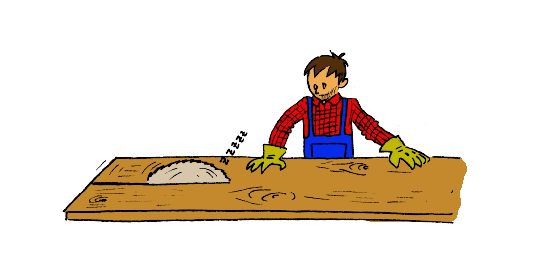
\includegraphics[width=5cm]{menuisier} \end{center}

Complète alors l'égalité $478,8 = 9 \cdot \ldots + \ldots$ . \label{NbEntDec_Approf81Qa}

 \item En utilisant la division écrite au \ref{NbEntDec_Approf81Qa}, recopie et complète les égalités suivantes :
 \begin{itemize}  
  \item $47,88 = 9 \cdot 5,3 + \ldots$ ;
  \item $4 788 = 9 \cdot 532 + \ldots$ ;
  \item $4 788 = 90 \cdot 53 + \ldots$ ;
  \item $4,788 = 9 \cdot \ldots + 0,018$.
  \end{itemize}
 \end{enumerate}
\end{exercice}


\begin{exercice}[Paquets empilés]
On a reçu au collège 7 rames de 500 feuilles pour la photocopieuse et 3 paquets de 24 pièces de « carton plume » :
\begin{enumerate}
 \item L'épaisseur d'une feuille de papier pour photocopieuse est de 0,11 mm et celle d'une pièce de « carton plume » est de 5 mm. Calcule un ordre de grandeur de la hauteur totale de tous ces paquets empilés ;
 \item Écris la hauteur totale des paquets en une seule expression puis calcule‑la.
 \end{enumerate}
\end{exercice}


\begin{exercice}[Densité de population]
On considère le tableau suivant :

\begin{center}
\begin{tabularx}{\linewidth}{|c|*{6}{>{\centering \arraybackslash}X|}}
\hline \rowcolor{U1} Continent & Nombre d'habitants & Superficie en km\up{2} \\
\hline \rowcolor{A3} Afrique & 965 millions & 30\,206\,704 \\
\hline \rowcolor{A3} Amérique & 911 millions & 42\,189\,120 \\
\hline \rowcolor{A3} Asie & 4,03 milliards & 43\,810\,582 \\
\hline \rowcolor{A3} Europe & 731 millions & 10\,180\,000 \\
\hline \rowcolor{A3} Océanie & 34 millions & 9\,008\,458 \\
\hline
\end{tabularx} \\
\end{center}

\begin{enumerate}
 \item Quel est le continent qui a le plus grand nombre d'habitants ? Et le plus petit nombre ?
 \item Quel est le continent qui a la plus grande superficie ? Et la plus petite ?
 \item Pour chaque continent, calcule la densité de population exprimée en habitants par km\up{2}. Tu donneras une valeur approchée à l'unité. 
 \item Ces résultats sont‑ils surprenants ? Explique.
 \item Calcule le nombre moyen d'habitants au km\up{2} dans le monde. Indique les continents qui sont en dessous de cette moyenne et ceux qui sont au dessus. 
 \end{enumerate}
\end{exercice}


\begin{exercice}[Football]
Le match de football entre le FC Barcelone et le Milan AC a eu lieu mardi soir 1\up{er} novembre à Barcelone. 
\begin{enumerate}
 \item Sachant qu’un match de football se joue en 2 mi-temps de 45 minutes séparées par une pause de 15 minutes, qu’il y a eu en tout 4 minutes d’arrêt de jeu en première mi-temps et 3 minutes en seconde mi-temps et que la rencontre a débuté à 20h45, trouver l’heure à laquelle le match s’est terminé. 
 \item Yvan, joueur de FC Barcelone est sorti du terrain au bout de 22 minutes de jeu en deuxième mi-temps, calculer l’heure à laquelle ce changement a eu lieu.
 \item Les supporters du Milan AC, qui avaient effectué le déplacement en autocar ont quitté le stade à 23h15 min. Sachant que leur voyage de retour a duré 16h40, calculer l’heure exacte et la date précise à laquelle ils sont arrivés à Milan. 
 \end{enumerate}
\end{exercice}